%package list
\documentclass{article}
\usepackage[top=3cm, bottom=3cm, outer=3cm, inner=3cm]{geometry}
\usepackage{multicol}
\usepackage{graphicx}
\usepackage{url}
%\usepackage{cite}
\usepackage{hyperref}
\usepackage{array}
%\usepackage{multicol}
\newcolumntype{x}[1]{>{\centering\arraybackslash\hspace{0pt}}p{#1}}
\usepackage{natbib}
\usepackage{pdfpages}
\usepackage{multirow}    
\usepackage[normalem]{ulem}
\useunder{\uline}{\ul}{}
\usepackage{svg}
\usepackage{xcolor}
\usepackage{listings}
\usepackage{amsmath}
\lstdefinestyle{ascii-tree}{
    literate={├}{|}1 {─}{--}1 {└}{+}1 
  }

\lstset{basicstyle=\ttfamily,
  showstringspaces=false,
  commentstyle=\color{red},
  keywordstyle=\color{blue}
}
%\usepackage{booktabs}
\usepackage{caption}
\usepackage{subcaption}
\usepackage{float}
\usepackage{array}

\usepackage{enumitem}


\newcolumntype{M}[1]{>{\centering\arraybackslash}m{#1}}
\newcolumntype{N}{@{}m{0pt}@{}}


%%%%%%%%%%%%%%%%%%%%%%%%%%%%%%%%%%%%%%%%%%%%%%%%%%%%%%%%%%%%%%%%%%%%%%%%%%%%
%%%%%%%%%%%%%%%%%%%%%%%%%%%%%%%%%%%%%%%%%%%%%%%%%%%%%%%%%%%%%%%%%%%%%%%%%%%%
\newcommand{\itemEmail}{vmaldonadov@unsa.edu.pe}
\newcommand{\itemStudent}{Victor Gonzalo Maldonado Vilca}
\newcommand{\itemCourse}{Programación Web 2}
\newcommand{\itemCourseCode}{1702122}
\newcommand{\itemSemester}{III}
\newcommand{\itemUniversity}{Universidad Nacional de San Agustín de Arequipa}
\newcommand{\itemFaculty}{Facultad de Ingeniería de Producción y Servicios}
\newcommand{\itemDepartment}{Departamento Académico de Ingeniería de Sistemas e Informática}
\newcommand{\itemSchool}{Escuela Profesional de Ingeniería de Sistemas}
\newcommand{\itemAcademic}{2024 - A}
\newcommand{\itemInput}{Del 23 de mayo de 2024}
\newcommand{\itemOutput}{Al 24 de junio de 2024}
\newcommand{\itemPracticeNumber}{09}
\newcommand{\itemTheme}{Django 5}
%%%%%%%%%%%%%%%%%%%%%%%%%%%%%%%%%%%%%%%%%%%%%%%%%%%%%%%%%%%%%%%%%%%%%%%%%%%%
%%%%%%%%%%%%%%%%%%%%%%%%%%%%%%%%%%%%%%%%%%%%%%%%%%%%%%%%%%%%%%%%%%%%%%%%%%%%

\usepackage[english,spanish]{babel}
\usepackage[utf8]{inputenc}
\AtBeginDocument{\selectlanguage{spanish}}
\renewcommand{\figurename}{Figura}
\renewcommand{\refname}{Referencias}
\renewcommand{\tablename}{Tabla} %esto no funciona cuando se usa babel
\AtBeginDocument{%
	\renewcommand\tablename{Tabla}
}

\usepackage{fancyhdr}
\pagestyle{fancy}
\fancyhf{}
\setlength{\headheight}{30pt}
\renewcommand{\headrulewidth}{1pt}
\renewcommand{\footrulewidth}{1pt}
\fancyhead[L]{\raisebox{-0.2\height}{
\includegraphics[width=3cm]{img/logo_episunsa.png}}}
\fancyhead[C]{\fontsize{7}{7}\selectfont	\itemUniversity \\ \itemFaculty \\ \itemDepartment \\ \itemSchool \\ \textbf{\itemCourse}}
\fancyhead[R]{\raisebox{-0.2\height}{
\includegraphics[width=1.2cm]{img/logo_abet}}}
\fancyfoot[L]{Victor M.}
\fancyfoot[C]{\itemCourse}
\fancyfoot[R]{Página \thepage}

% para el codigo fuente
\usepackage{listings}
\usepackage{color, colortbl}
\definecolor{dkgreen}{rgb}{0,0.6,0}
\definecolor{gray}{rgb}{0.5,0.5,0.5}
\definecolor{mauve}{rgb}{0.58,0,0.82}
\definecolor{codebackground}{rgb}{0.95, 0.95, 0.92}
\definecolor{tablebackground}{rgb}{0.8, 0, 0}
\definecolor{gitgreen}{RGB}{40, 160, 40}
\definecolor{gitred}{RGB}{255, 0, 0}
\definecolor{gitgray}{RGB}{128, 128, 128}

\lstset{frame=tb,
	language=bash,
	aboveskip=3mm,
	belowskip=3mm,
	showstringspaces=false,
	columns=flexible,
	basicstyle={\small\ttfamily},
	numbers=none,
	numberstyle=\tiny\color{gray},
	keywordstyle=\color{blue},
	commentstyle=\color{dkgreen},
	stringstyle=\color{mauve},
	breaklines=true,
	breakatwhitespace=true,
	tabsize=3,
	backgroundcolor= \color{codebackground},
}

\begin{document}
	
	\vspace*{10px}
	
	\begin{center}	
		\fontsize{17}{17} \textbf{ Informe de Django 05}
	\end{center}
	\centerline{\textbf{\Large Tema: \itemTheme}}
	%\vspace*{0.5cm}	

	\begin{flushright}
		\begin{tabular}{|M{2.5cm}|N|}
			\hline 
			\rowcolor{tablebackground}
			\color{white} \textbf{Nota}  \\
			\hline 
			     \\[30pt]
			\hline 			
		\end{tabular}
	\end{flushright}	

	\begin{table}[H]
		\begin{tabular}{|x{4.7cm}|x{4.8cm}|x{4.8cm}|}
			\hline 
			\rowcolor{tablebackground}
			\color{white} \textbf{Estudiante} & \color{white}\textbf{Escuela}  & \color{white}\textbf{Asignatura}   \\
			\hline 
			{\itemStudent \par \itemEmail} & \itemSchool & {\itemCourse \par Semestre: \itemSemester \par Código: \itemCourseCode}     \\
			\hline 			
		\end{tabular}
	\end{table}		
	
	\begin{table}[H]
		\begin{tabular}{|x{4.7cm}|x{4.8cm}|x{4.8cm}|}
			\hline 
			\rowcolor{tablebackground}
			\color{white}\textbf{Tarea} & \color{white}\textbf{Tema}  & \color{white}\textbf{Duración}   \\
			\hline 
			\itemPracticeNumber & \itemTheme & 2 horas   \\
			\hline 
		\end{tabular}
	\end{table}
	
	\begin{table}[H]
		\begin{tabular}{|x{4.7cm}|x{4.8cm}|x{4.8cm}|}
			\hline 
			\rowcolor{tablebackground}
			\color{white}\textbf{Semestre académico} & \color{white}\textbf{Fecha de inicio}  & \color{white}\textbf{Fecha de entrega}   \\
			\hline 
			\itemAcademic & \itemInput &  \itemOutput  \\
			\hline 
		\end{tabular}
	\end{table}
  
%%%%%%%%%%%%%%%%%%%%
 
	\section{Tarea}
  \begin{itemize}
    \item Repetir las actividades vistas en teoria de Django5.  Ir haciendo commits cada avance.  Compartirlo con el docente (CarloCorrales010)
  \end{itemize}
  
%%%%%%%%%%%%%%%%%%%% 
 
  \section{Entregables}
  \begin{itemize}
    \item Informe hecho en Latex.
    \item Captura de pantalla del siguiente comando:
    \begin{lstlisting}[language=bash]
      git log --graph --pretty=oneline --abbrev-commit --all
    \end{lstlisting}
    \item URL - Repositorio GitHub
  \end{itemize}
  
%%%%%%%%%%%%%%%%%%%%    
		
	\section{Equipos, materiales y temas utilizados}
  \begin{itemize}
    \item Configuración de Proyectos
    \item Modelado de Datos
    \item Migraciones de Base de Datos
    \item Desarrollo de Vistas y URLs
    \item Uso de Plantillas HTML
    \item Administración de Aplicaciones
    \item Control de Versiones
    \item Creacion y manejo de Formularios
    \item Uso de Vistas Genericas
    \item Archivos estaticos
  \end{itemize}

%%%%%%%%%%%%%%%%%%%%

	\section{Captura de Pantalla}
  \begin{figure}[H]
    \centering
    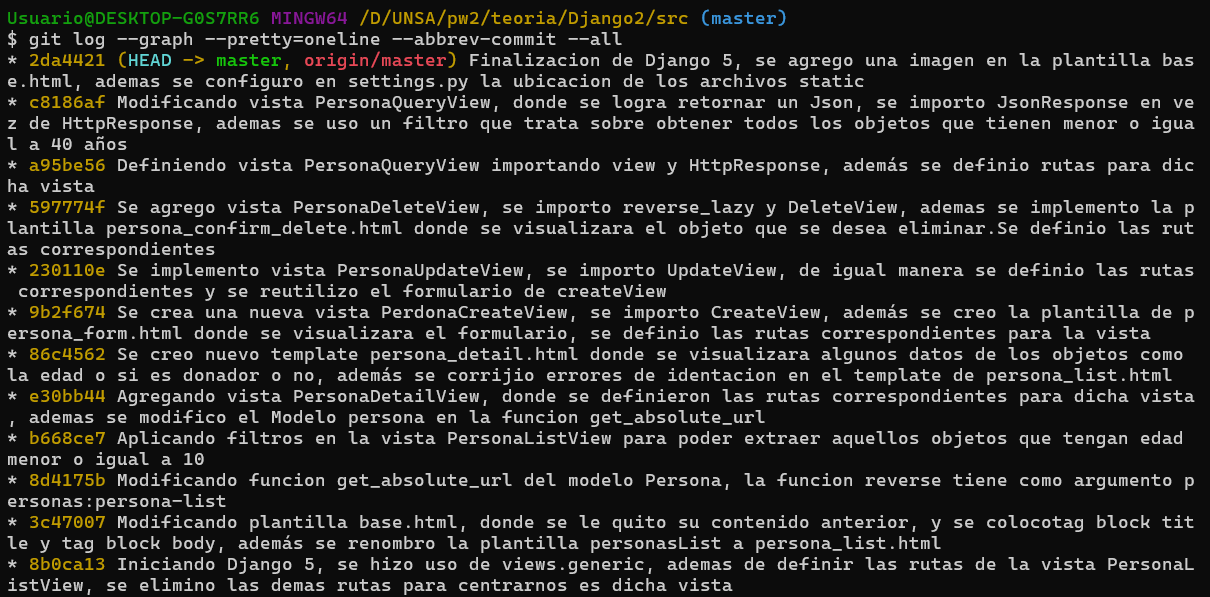
\includegraphics[width=1\textwidth, keepaspectratio]{img/commits1.png}
    \caption{commits - local}
  \end{figure}

%%%%%%%%%%%%%%%%%%%%

  \section{URL de Repositorio Github}
  \begin{itemize}
    \item URL del Repositorio GitHub.
    \item \url{https://github.com/Victor-Gonzalo-Maldonado-Vilca/Django2.git}
  \end{itemize}

%%%%%%%%%%%%%%%%%%%%

  \section{Desarrollo del trabajo}
  \textit{Continuamos a partir del proyecto realizado en Django 4}
  
%%%%%%%%%%%%

  \subsection{Imágenes de Ejecución}
  \begin{figure}[H]
    \centering
    \fbox{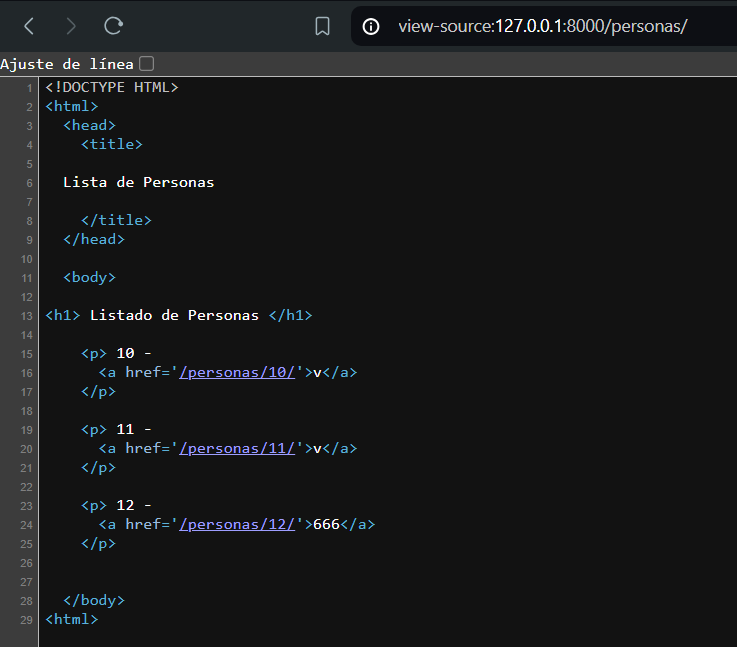
\includegraphics[width=1\textwidth, keepaspectratio]{img/viewsource.png}}
    \caption{View Source}
  \end{figure}
  \begin{figure}[H]
    \centering
    \fbox{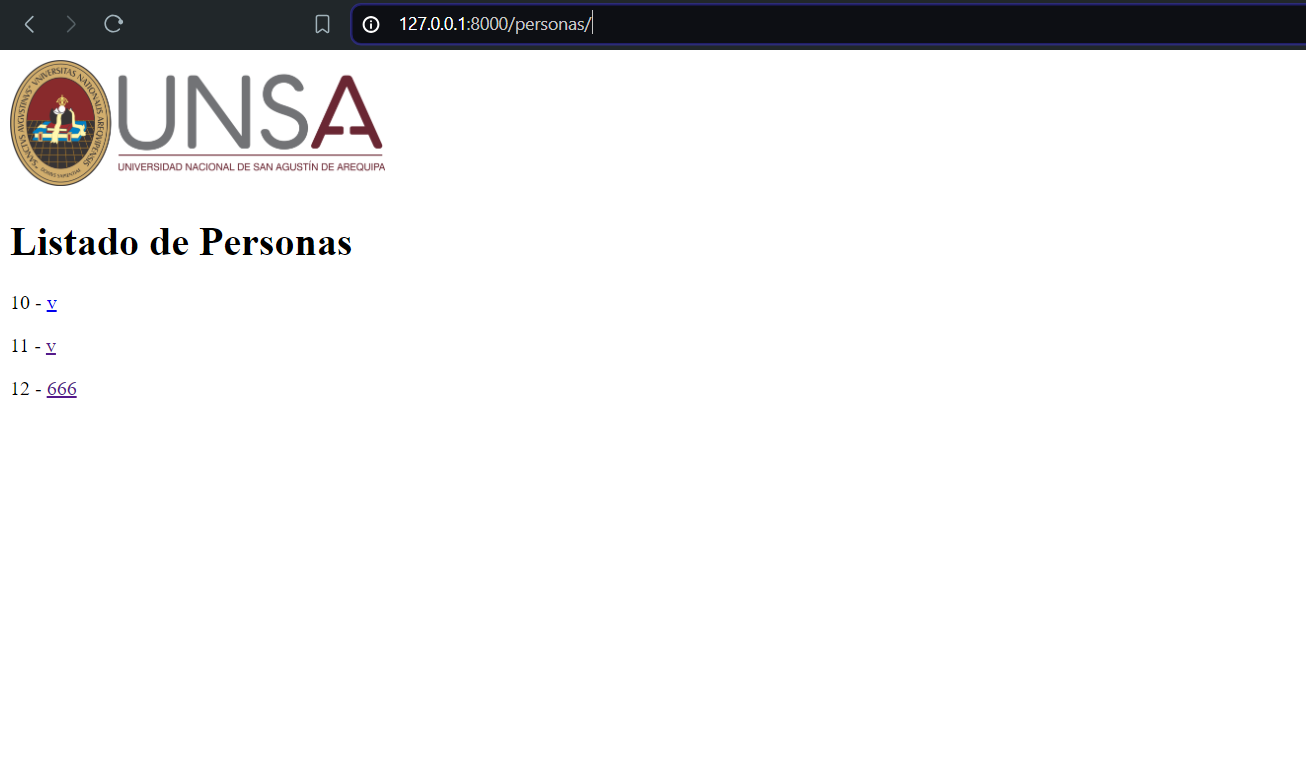
\includegraphics[width=1\textwidth, keepaspectratio]{img/ejecucion1.png}}
    \caption{Listar Objetos}
  \end{figure}
  \begin{figure}[H]
    \centering
    \fbox{
\includegraphics[width=1\textwidth, keepaspectratio]{img/ejecucion2.png}}
    \caption{Detallar Objetos}
  \end{figure}
  \begin{figure}[H]
    \centering
    \fbox{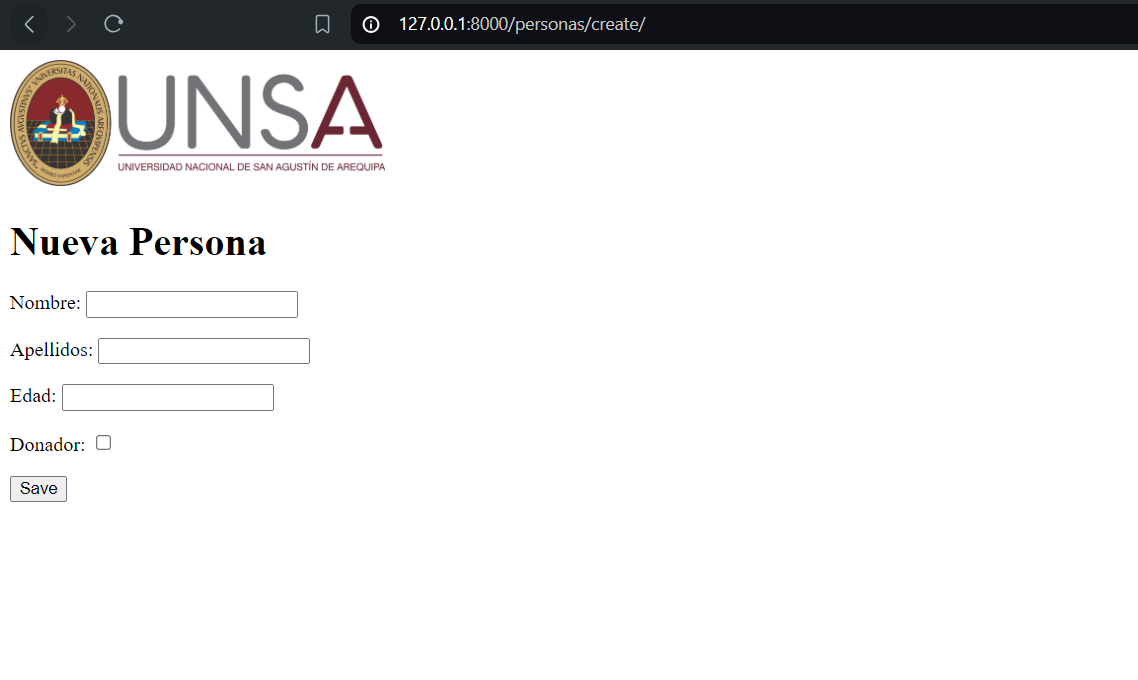
\includegraphics[width=1\textwidth, keepaspectratio]{img/ejecucion3.png}}
    \caption{Agregar Objetos}
  \end{figure}
  \begin{figure}[H]
    \centering
    \fbox{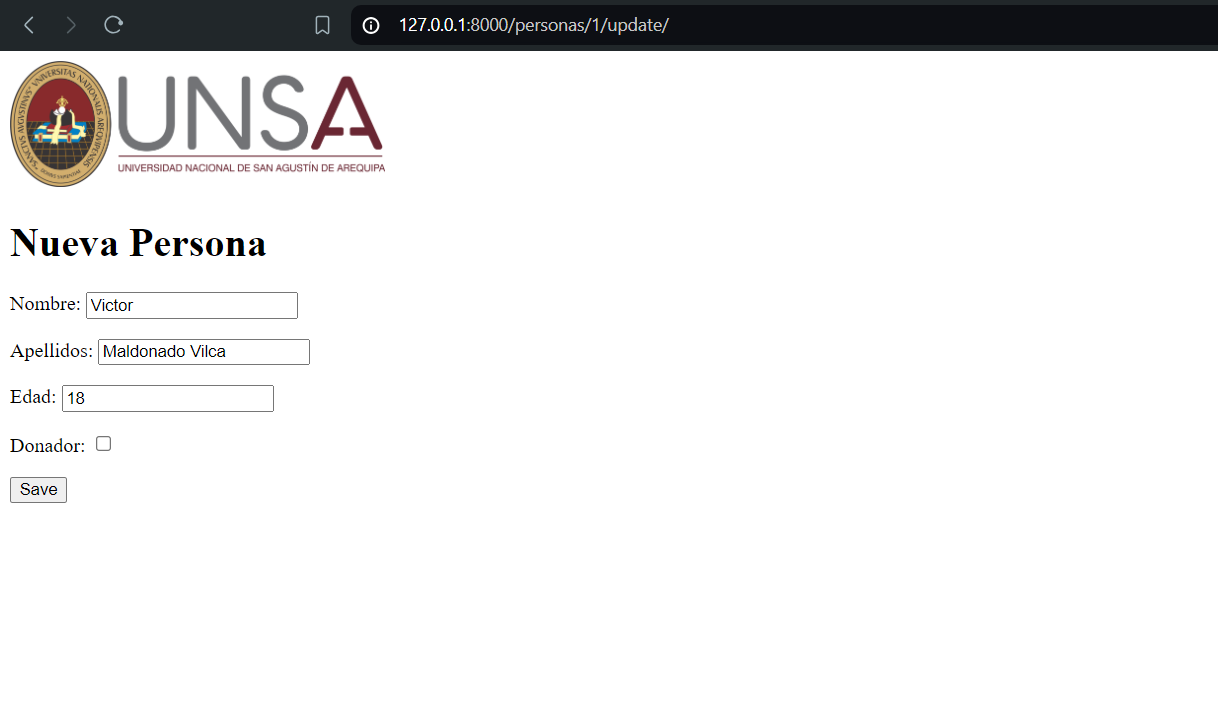
\includegraphics[width=1\textwidth, keepaspectratio]{img/ejecucion4.png}}
    \caption{Actualizar Objetos}
  \end{figure}
  \begin{figure}[H]
    \centering
    \fbox{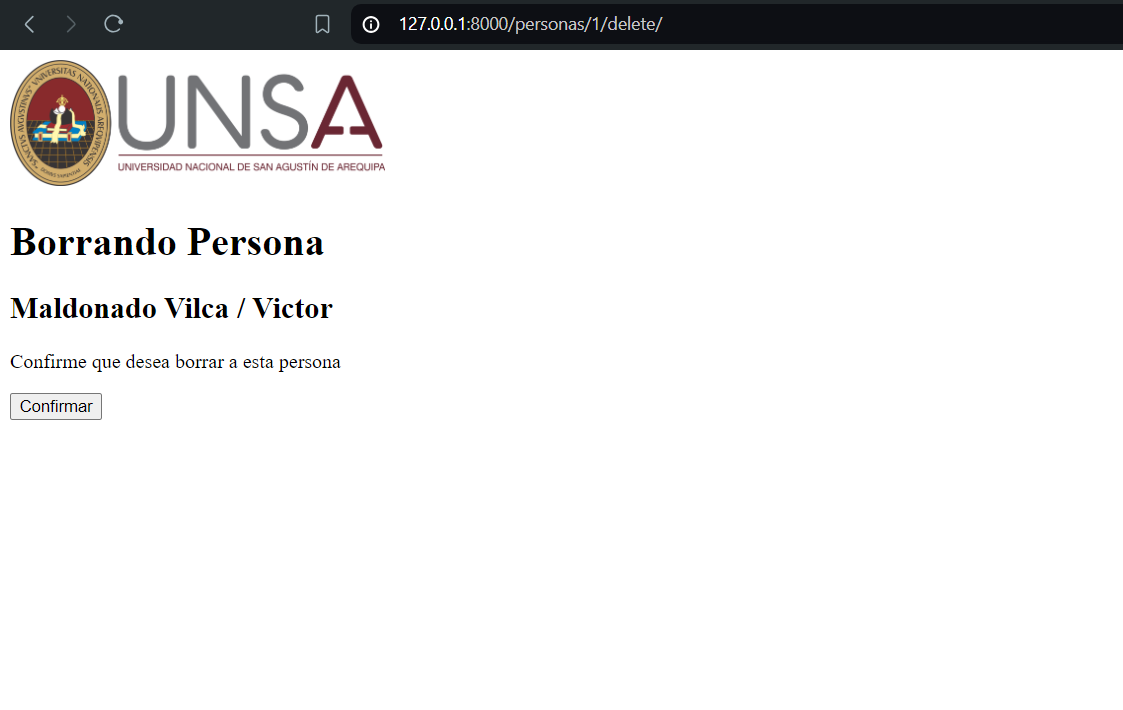
\includegraphics[width=1\textwidth, keepaspectratio]{img/ejecucion5.png}}
    \caption{Borrar Objetos}
  \end{figure}
  \begin{figure}[H]
    \centering
    \fbox{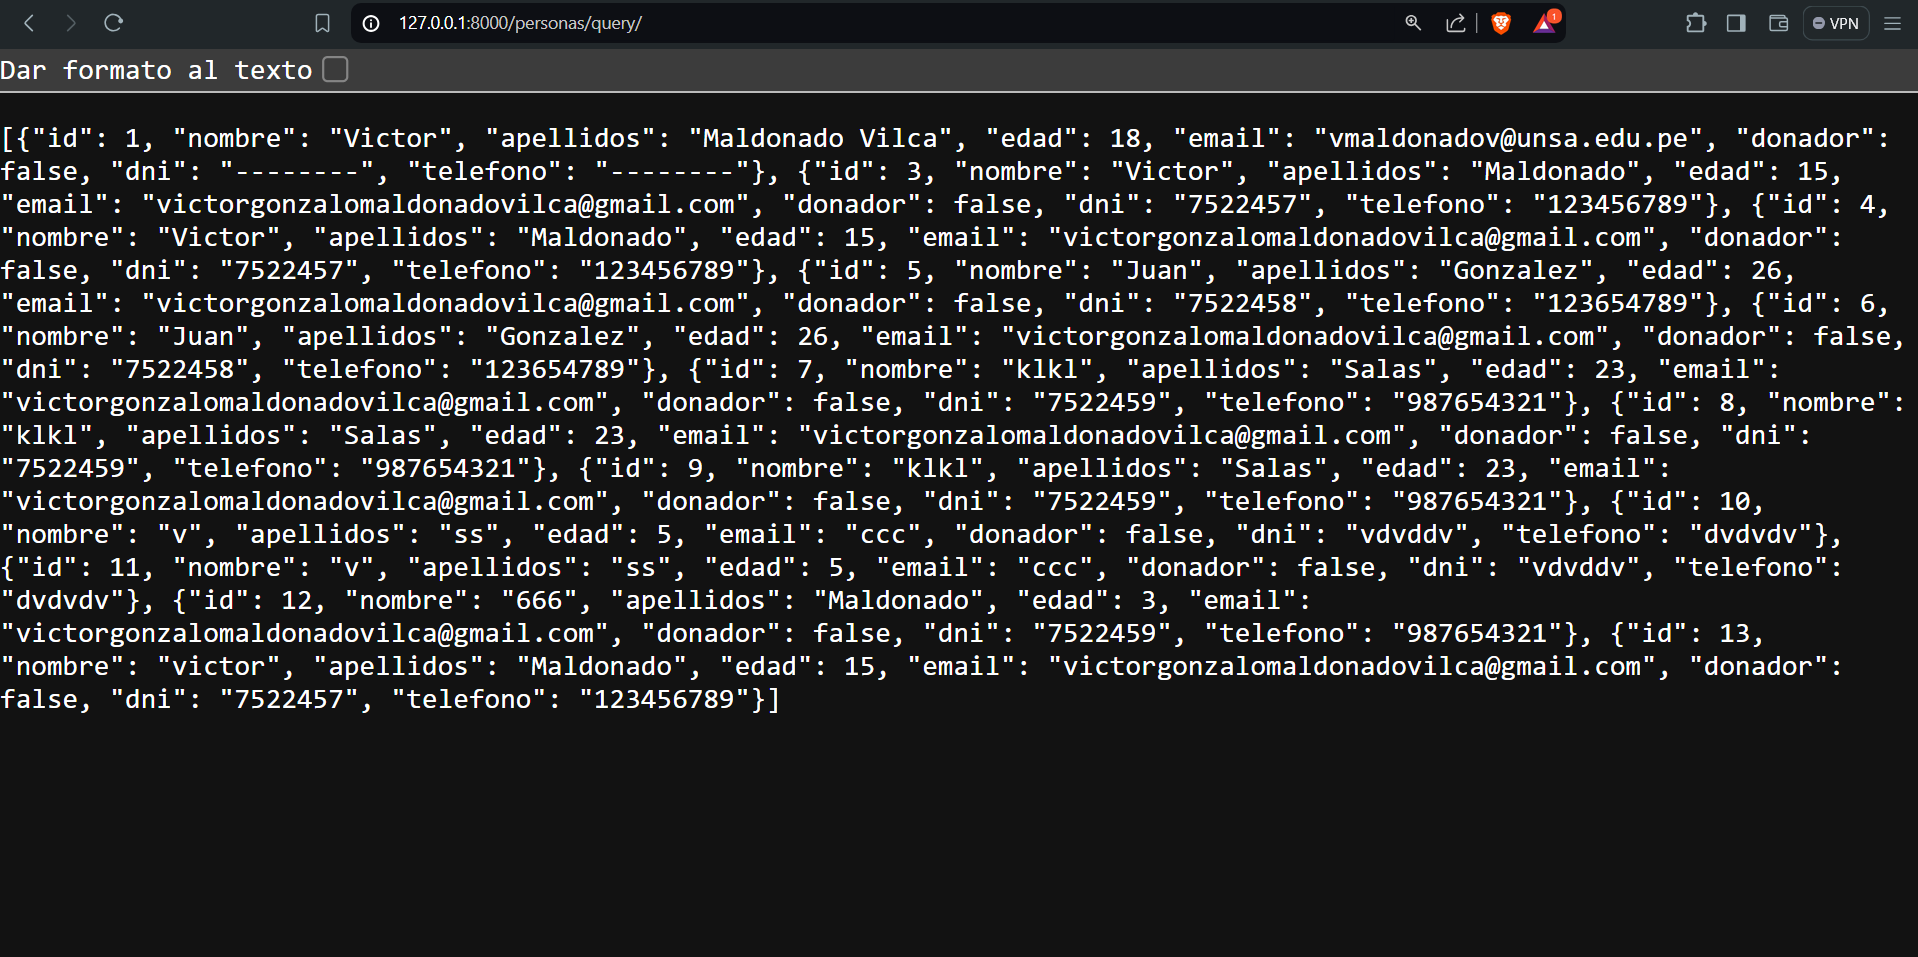
\includegraphics[width=1\textwidth, keepaspectratio]{img/ejecucion6.png}}
    \caption{JSON de los Objetos - query}
  \end{figure}
  
%%%%%%%%%%%%

  \subsection{Modelos -- Aplicación personas}
  Esta función $\text{get\_absolute\_url}$ genera la URL absoluta para una instancia del modelo utilizando el nombre de la 
  ruta personas:persona-detail y el identificador primario (pk) del objeto. Esto permite obtener una URL directa 
  para visualizar los detalles de la instancia correspondiente.
  \begin{lstlisting}[language=Python, caption={Modelo Persona}]
    def get_absolute_url(self):
      return reverse('personas:persona-detail', kwargs = {'pk': self.id})
  \end{lstlisting}
    
%%%%%%%%%%%%

  \subsection{Vistas -- Aplicación personas}
  
%%%%%%
  
  \subsubsection{Importaciones}
  Se importa render desde django.shortcuts para renderizar plantillas HTML. Se importa $\text{reverse\_lazy}$ desde django.urls 
  para la construcción de URLs reversibles y JsonResponse desde django.http para devolver respuestas JSON. Las vistas 
  genéricas ListView, DetailView, CreateView, UpdateView, DeleteView y View se importan desde django.views.generic para 
  manejar las diferentes operaciones CRUD y vistas personalizadas. Finalmente, se importa el modelo Persona desde .models 
  para interactuar con los datos del modelo en las vistas.
  \begin{lstlisting}[language=Python]
    from django.shortcuts import render
    from django.urls import reverse_lazy
    from django.http import JsonResponse
    from django.views.generic import (
        ListView,
        DetailView,
        CreateView,
        UpdateView,
        DeleteView,
        View,
        )
    from .models import Persona
  \end{lstlisting} 
  
%%%%%%
  
  \subsubsection{Vista PersonaQueryView()}
  \begin{itemize}
    \item \textbf{Descripción: }
    \begin{itemize}
      \item Esta vista personalizada hereda de View y define el método get.
      \item Filtra las instancias del modelo Persona cuya edad es menor o igual a 40.
      \item Retorna un JsonResponse con los datos de las instancias filtradas en formato JSON.
    \end{itemize}
    \item \textbf{Código: }
    \begin{lstlisting}[language=Python]
      class PersonaQueryView(View):
        def get(self, request, *args, **kwargs):
          queryset = Persona.objects.filter(edad__lte='40')
          return JsonResponse(list(queryset.values()), safe = False) 
    \end{lstlisting}   
  \end{itemize}
  \newpage
  
%%%%%%
  
  \subsubsection{Vista PersonaDetailView()}
  \begin{itemize}
    \item \textbf{Descripción: }
    \begin{itemize}
      \item Esta vista hereda de DetailView y se usa para mostrar los detalles de una instancia específica del modelo Persona.
      \item Django automáticamente busca una plantilla llamada $\text{personaí\_detail.html}$ y pasa la instancia del modelo a esta plantilla.
    \end{itemize}
    \item \textbf{Código: }
    \begin{lstlisting}[language=Python]
      class PersonaDetailView(DetailView):
        model = Persona
    \end{lstlisting}   
  \end{itemize}
  
%%%%%%
  
  \subsubsection{Vista PersonaListView()}
  \begin{itemize}
    \item \textbf{Descripción: }
    \begin{itemize}
      \item Hereda de ListView y se utiliza para mostrar una lista de instancias del modelo Persona
      \item Filtra las instancias cuya edad es menor o igual a 40.
      \item Django busca una plantilla llamada $\text{persona\_list.html}$ y pasa la lista de instancias a esta plantilla.
    \end{itemize}
    \item \textbf{Código: }
    \begin{lstlisting}[language=Python]
      class PersonaListView(ListView):
        model = Persona
        queryset = Persona.objects.filter(edad__lte='40')
    \end{lstlisting}   
  \end{itemize}
  
%%%%%%
  
  \subsubsection{Vista PersonaCreateView()}
  \begin{itemize}
    \item \textbf{Descripción: }
    \begin{itemize}
      \item Hereda de CreateView y se utiliza para crear nuevas instancias del modelo Persona.
      \item Define los campos del modelo que estarán disponibles en el formulario de creación.
      \item Django busca una plantilla llamada $\text{persona\_form.html}$ para renderizar el formulario.
    \end{itemize}
    \item \textbf{Código: }
    \begin{lstlisting}[language=Python]
      class PersonaCreateView(CreateView):
        model = Persona
        fields = [
            'nombre',
            'apellidos',
            'edad',
            'donador',
        ]
    \end{lstlisting}   
  \end{itemize}
  
%%%%%%
  
  \subsubsection{Vista PersonaUpdateView()}
  \begin{itemize}
    \item \textbf{Descripción: }
    \begin{itemize}
      \item Hereda de UpdateView y se utiliza para actualizar instancias existentes del modelo Persona.
      \item Define los campos del modelo que estarán disponibles en el formulario de actualización.
      \item Django busca una plantilla llamada $\text{persona\_form.html}$ para renderizar el formulario de actualización.
    \end{itemize}
    \item \textbf{Código: }
    \begin{lstlisting}[language=Python]
      class PersonaUpdateView(UpdateView):
        model = Persona
        fields = [
            'nombre',
            'apellidos',
            'edad',
            'donador',
        ]
    \end{lstlisting}   
  \end{itemize}
  
%%%%%%
  
  \subsubsection{Vista PersonaDeleteView()}
  \begin{itemize}
    \item \textbf{Descripción: }
    \begin{itemize}
      \item Hereda de DeleteView y se utiliza para eliminar instancias del modelo Persona.
      \item Define $\text{success\_url}$ para redirigir a la lista de personas después de eliminar una instancia.
      \item Django busca una plantilla llamada $\text{persona\_confirm\_delete.html}$ para confirmar la eliminación.
    \end{itemize}
    \item \textbf{Código: }
    \begin{lstlisting}[language=Python]
      class PersonaDeleteView(DeleteView):
        model = Persona
        success_url = reverse_lazy('personas:persona-list')
    \end{lstlisting}   
  \end{itemize}
  
%%%%%%%%%%%%

  \subsection{URLs}
  
%%%%%%
  
  \subsubsection{urls del proyecto listaContactos}
  \begin{itemize}
    \item \textbf{Descripción: }Este archivo urls.py principal de un proyecto Django define las rutas URL que gestionan las solicitudes. 
    Importa módulos necesarios y vistas, aunque no se usan en este archivo. La lista urlpatterns contiene rutas que emparejan 
    solicitudes con vistas: path('admin/', admin.site.urls) para la interfaz de administración accesible a través de /admin/, 
    y path('personas/', include('personas.urls')) para incluir las rutas definidas en la aplicación personas, accesibles a 
    través de /personas/
    \item \textbf{Código: }
    \begin{lstlisting}[language=Python]
      from django.contrib import admin
      from django.urls import path, include
      from inicio.views import myHomeView, anotherView

      urlpatterns = [
        path('admin/', admin.site.urls),
        path('personas/', include('personas.urls')),
      ]
    \end{lstlisting}   
  \end{itemize}
  
%%%%%%
  
  \subsubsection{urls de la aplicación personas}
  \begin{itemize}
    \item \textbf{Descripción: }Se define las rutas URL específicas para la aplicación personas. Se importan las vistas 
    necesarias desde personas.views y se asigna el nombre de la aplicación como personas. La lista urlpatterns contiene 
    las siguientes rutas: path('') para la lista de personas con PersonaListView, path('<int:pk>/') para el detalle de 
    una persona con PersonaDetailView, path('create/') para la creación de una nueva persona con PersonaCreateView, 
    path('<int:pk>/update/') para la actualización de una persona existente con PersonaUpdateView, path('<int:pk>/delete/') 
    para la eliminación de una persona con PersonaDeleteView, y path('query/') para consultar personas según ciertos criterios 
    con PersonaQueryView.
    \item \textbf{Código: }
    \begin{lstlisting}[language=Python]
      from django.urls import path
      from personas.views import (
          PersonaListView,
          PersonaDetailView,
          PersonaCreateView,
          PersonaUpdateView,
          PersonaDeleteView,
          PersonaQueryView,
          )

      app_name = 'personas'
      urlpatterns = [
          path('', PersonaListView.as_view(), name = 'persona-list'),
          path('<int:pk>/', PersonaDetailView.as_view(), name = 'persona-detail'),
          path('create/', PersonaCreateView.as_view(), name = 'persona-create'),
          path('<int:pk>/update/', PersonaUpdateView.as_view(), name = 'persona-update'),
          path('<int:pk>/delete/', PersonaDeleteView.as_view(), name = 'persona-delete'),
          path('query/', PersonaQueryView.as_view(), name = 'persona-query'),
      ]
    \end{lstlisting}   
  \end{itemize}

%%%%%%%%%%%%%%%%%%%%%

  \section{Templates}
  \textit{En esta actividad se realizo 5 templates}
  
%%%%%%%%%%%%

  \subsection{Plantilla modificada base.html}
  \begin{itemize}
    \item \textbf{Descripción: }La siguiente plantilla HTML utiliza load static para cargar archivos estáticos como CSS, 
    imágenes, etc. El bloque block title define el título de la página, que puede ser reemplazado en las plantillas que 
    heredan de esta. El bloque block body se utiliza para el contenido principal de la página, que también puede ser 
    reemplazado en las plantillas que heredan de esta. El código static "personas/logo-unsa.png" se utiliza para cargar 
    la imagen del logo de la UNSA desde los archivos estáticos.
    \item \textbf{Código: }
    \begin{lstlisting}[language=html]
      
      <!DOCTYPE HTML>
      <html>
        <head>
          <title>
            
            
          </title>
        </head>
        
        <body>
          <img src='' width='300px' alt='logo unsa'> 
          
          
        </body>
      </html>
    \end{lstlisting}   
  \end{itemize}
  
%%%%%%%%%%%%

  \subsection{Plantilla $\text{persona\_list.html}$}
  \begin{itemize}
    \item \textbf{Descripción: }Esta plantilla HTML extiende de 'base.html'. En el bloque block title, 
    se define el título de la página como "Lista de Personas". En el bloque block body, se muestra un encabezado 
    $\textbf{\<h1\>}$ con el texto "Listado de Personas", seguido de un bucle for instance in $\text{object\_list}$ que 
    itera sobre una lista de objetos instance y muestra su ID y nombre en párrafos $\text{\<p\>}$. Cada nombre es un enlace a la URL 
    definida por $\text{get\_absolute\_url}$ para ese objeto.
    \item \textbf{Código: }
    \begin{lstlisting}[language=html]
      
      
        Lista de Personas
      
      
      <h1> Listado de Personas </h1>
      
          <p> {{instance.id}} - 
            <a href='{{instance.get_absolute_url}}'>{{instance.nombre}}</a>
          </p>
      
      
    \end{lstlisting}   
  \end{itemize}
  
%%%%%%%%%%%%

  \subsection{Plantilla $\text{persona\_detail.html}$}
  \begin{itemize}
    \item \textbf{Descripción: }Este es un archivo de plantilla HTML que extiende de 'base.html'. 
    En el bloque block title, se define el título de la página como "Detalle de Personas". 
    En el bloque block body, se muestra un encabezado $\text{\<h1\>}$ con el texto "Detalle de Personas", 
    seguido de un encabezado $\text{\<h2\>}$ que muestra los apellidos y nombres del objeto object. Luego, se 
    muestra la edad del objeto y un mensaje que indica si es donador de órganos o no, dependiendo del valor de object.donador.
    \item \textbf{Código: }
    \begin{lstlisting}[language=html]
      
      
        Detalle de Personas
      
      
      <h1> Detalle de Personas </h1>
      <h2> {{ object.apellidos }} / {{ object.nombres }}</h2>
      <p>{{ object.edad }} .... de edad.</p>
      <p>
      
        Es
      
        No es
      
        donador de organos
      </p>
      
    \end{lstlisting}   
  \end{itemize}
  
%%%%%%%%%%%%

  \subsection{Plantilla $\text{persona\_form.html}$}
  \begin{itemize}
    \item \textbf{Descripción: }Este archivo de plantilla HTML extiende de 'base.html' y define el título de la página como 
    "Nueva Persona" en el bloque block title. En el bloque block body, se muestra un encabezado $\text{\<h1\>}$
    con el texto "Nueva Persona", seguido de un formulario que utiliza el método POST y el token CSRF para seguridad. 
    El formulario renderiza los campos del formulario form utilizando {{ $\text{form.as\_p}$ }} y agrega un botón "Save" para 
    enviar el formulario.
    \item \textbf{Código: }
    \begin{lstlisting}[language=html]
      
      
        Nueva Persona
      
      
      <h1> Nueva Persona </h1>
      <form method='post'>
        {{ form.as_p }}
        <input type="submit" value="Save">
      </form>
      
    \end{lstlisting}   
  \end{itemize}
  
%%%%%%%%%%%%

  \subsection{Plantilla $\text{persona\_confirm\_delete.html}$}
  \begin{itemize}
    \item \textbf{Descripción: }Se define una plantilla HTML que se extiende de 'base.html' y establece el título de la 
    página como "Borrando Persona" en el bloque block title. En el bloque block body, 
    se muestra un encabezado $\text{\<h1\>}$ con el texto "Borrando Persona", seguido de un subtítulo $\text{\<h2\>}$ que muestra 
    los apellidos y nombre de la persona a borrar. Luego, se presenta un formulario que utiliza el método POST 
    y el token CSRF para seguridad, con un mensaje de confirmación y un botón "Confirmar" para proceder con la 
    eliminación de la persona.
    \item \textbf{Código: }
    \begin{lstlisting}[language=html]
      
      
        Borrando Persona
      
      
      <h1> Borrando Persona </h1>
      <h2>{{ object.apellidos }} / {{ object.nombre }}</h2>
      <form method='post'>
        <p>
        Confirme que desea borrar a esta persona
        </p>
        <input type="submit" value="Confirmar">
      </form>
      
    \end{lstlisting}   
  \end{itemize}
  
%%%%%%%%%%%%

  \subsection{Ejecución del servidor}
  Este siguiente comando inicia el servidor local de Django. Una vez ejecutado, el servidor estará disponible por defecto en la dirección 
  \texttt{http://127.0.0.1:8000/}. Desde esta dirección, se puede acceder a las diferentes vistas y funcionalidades del 
  proyecto Django.
  \begin{lstlisting}[language=bash]
    python manage.py runserver
  \end{lstlisting}

%%%%%%%%%%%%%%%%%%%%

  \section{Conclusiones}
  \begin{itemize}
    \item El uso de archivos estáticos mejora la experiencia del usuario al permitir un diseño más atractivo y funcional.
    \item La compatibilidad con herramientas y frameworks como Django asegura una gestión eficiente de los archivos estáticos 
    para una experiencia web sólida y profesional.
    \item Se ha adquirido un conocimiento significativo en el desarrollo con Django, cubriendo aspectos importantes como 
    la configuración de URL, la definición de vistas y la creación de formularios.
    \item La comprensión de la estructura de los proyectos en Django, que incluye la organización de aplicaciones, modelos 
    y archivos de configuración, resulta fundamental para lograr un desarrollo eficiente.
    \item La utilización de herramientas como el servidor de desarrollo de Django y el sistema de plantillas ha facilitado 
    un desarrollo ágil y eficaz de la aplicación.
    \item Django se destaca como un framework web poderoso y versátil que permite la rápida y eficiente creación de aplicaciones web.
    \item La arquitectura MVC (Modelo-Vista-Controlador) de Django contribuye a organizar el código de manera estructurada y 
    modular, lo que favorece la mantenibilidad y escalabilidad de las aplicaciones.
    \item Con un sólido conocimiento de Django y al seguir las mejores prácticas de desarrollo, es posible crear aplicaciones 
    web robustas y de alto rendimiento.
  \end{itemize}
  
%%%%%%%%%%%%%%%%%%%%
	\newpage
	\subsection{\textcolor{red}{Rúbrica para el contenido del Informe y demostración}}
	\begin{itemize}			
		\item El alumno debe marcar o dejar en blanco en celdas de la columna \textbf{Checklist} si cumplio con el ítem correspondiente.
		\item Si un alumno supera la fecha de entrega,  su calificación será sobre la nota mínima aprobada, siempre y cuando cumpla con todos lo items.
		\item El alumno debe autocalificarse en la columna \textbf{Estudiante} de acuerdo a la siguiente tabla:
	
		\begin{table}[ht]
			\caption{Niveles de desempeño}
			\begin{center}
			\begin{tabular}{ccccc}
    			\hline
    			 & \multicolumn{4}{c}{Nivel}\\
    			\cline{1-5}
    			\textbf{Puntos} & Insatisfactorio 25\%& En Proceso 50\% & Satisfactorio 75\% & Sobresaliente 100\%\\
    			\textbf{2.0}&0.5&1.0&1.5&2.0\\
    			\textbf{4.0}&1.0&2.0&3.0&4.0\\
    		\hline
			\end{tabular}
		\end{center}
	\end{table}	
	

	\end{itemize}

 
	
	\begin{table}[H]
		\caption{Rúbrica para contenido del Informe y demostración}
		\setlength{\tabcolsep}{0.5em} % for the horizontal padding
		{\renewcommand{\arraystretch}{1.5}% for the vertical padding
		%\begin{center}
		\begin{tabular}{|p{2.7cm}|p{7cm}|x{1.3cm}|p{1.2cm}|p{1.5cm}|p{1.1cm}|}
			\hline
    		\multicolumn{2}{|c|}{Contenido y demostración} & Puntos & Checklist & Estudiante & Profesor\\
			\hline
			\textbf{1. GitHub} & Hay enlace URL activo del directorio para el  laboratorio hacia su repositorio GitHub con código fuente terminado y fácil de revisar. &2 &X &2 & \\ 
			\hline
			\textbf{2. Commits} &  Hay capturas de pantalla de los commits más importantes con sus explicaciones detalladas. (El profesor puede preguntar para refrendar calificación). &4 &X &4 & \\ 
			\hline 
			\textbf{3. Código fuente} &  Hay porciones de código fuente importantes con numeración y explicaciones detalladas de sus funciones. &2 &X &2 & \\ 
			\hline 
			\textbf{4. Ejecución} & Se incluyen ejecuciones/pruebas del código fuente  explicadas gradualmente. &2 &X &2 & \\ 
			\hline			
			\textbf{5. Pregunta} & Se responde con completitud a la pregunta formulada en la tarea.  (El profesor puede preguntar para refrendar calificación).  &2 &X &2 & \\ 
			\hline	
			\textbf{6. Fechas} & Las fechas de modificación del código fuente estan dentro de los plazos de fecha de entrega establecidos. &2 &X &2 & \\ 
			\hline 
			\textbf{7. Ortografía} & El documento no muestra errores ortográficos. &2 &X &2 & \\ 
			\hline 
			\textbf{8. Madurez} & El Informe muestra de manera general una evolución de la madurez del código fuente,  explicaciones puntuales pero precisas y un acabado impecable.   (El profesor puede preguntar para refrendar calificación).  &4 &X &4 & \\ 
			\hline
			\multicolumn{2}{|c|}{\textbf{Total}} &20 & &20 & \\ 
			\hline
		\end{tabular}
		%\end{center}
		%\label{tab:multicol}
		}
	\end{table}


%%%%%%%%%%%%%%%%%%%%%%%%%%%%%%%%%%%%%%%%%%%%%%%%%%%%%%%%%%%%%%%%%%%
	
  \newpage
  \section{Referencias}
  \begin{itemize}
    \item \url{https://docs.djangoproject.com/en/5.0/}
    \item \url{https://docs.github.com/es}
    \item \url{https://git-scm.com/doc}
  \end{itemize}
  
%%%%%%%%%%%%%%%%%%%% 
%\clearpage
%\bibliographystyle{apalike}
%\bibliographystyle{IEEEtranN}
%\bibliography{bibliography}
			
\end{document}
